\documentclass[tikz,border=12pt]{standalone}
\usepackage[T1]{fontenc}
\usepackage{mathpazo}
\usepackage{amsmath,amssymb}
\usetikzlibrary{arrows.meta, positioning, calc, fit, decorations.pathreplacing, matrix}
\definecolor{stblue}{HTML}{7B97AD}
\definecolor{rwgold}{HTML}{B8995E}
\definecolor{sage}{HTML}{7A9A7E}
\definecolor{dkbrown}{HTML}{3D3530}
\definecolor{wmgray}{HTML}{7B7067}
\definecolor{cream}{HTML}{F9F6F0}
\definecolor{border}{HTML}{D4C9B8}
\definecolor{terracotta}{HTML}{C47A6A}
\definecolor{lavender}{HTML}{907EA0}

\begin{document}
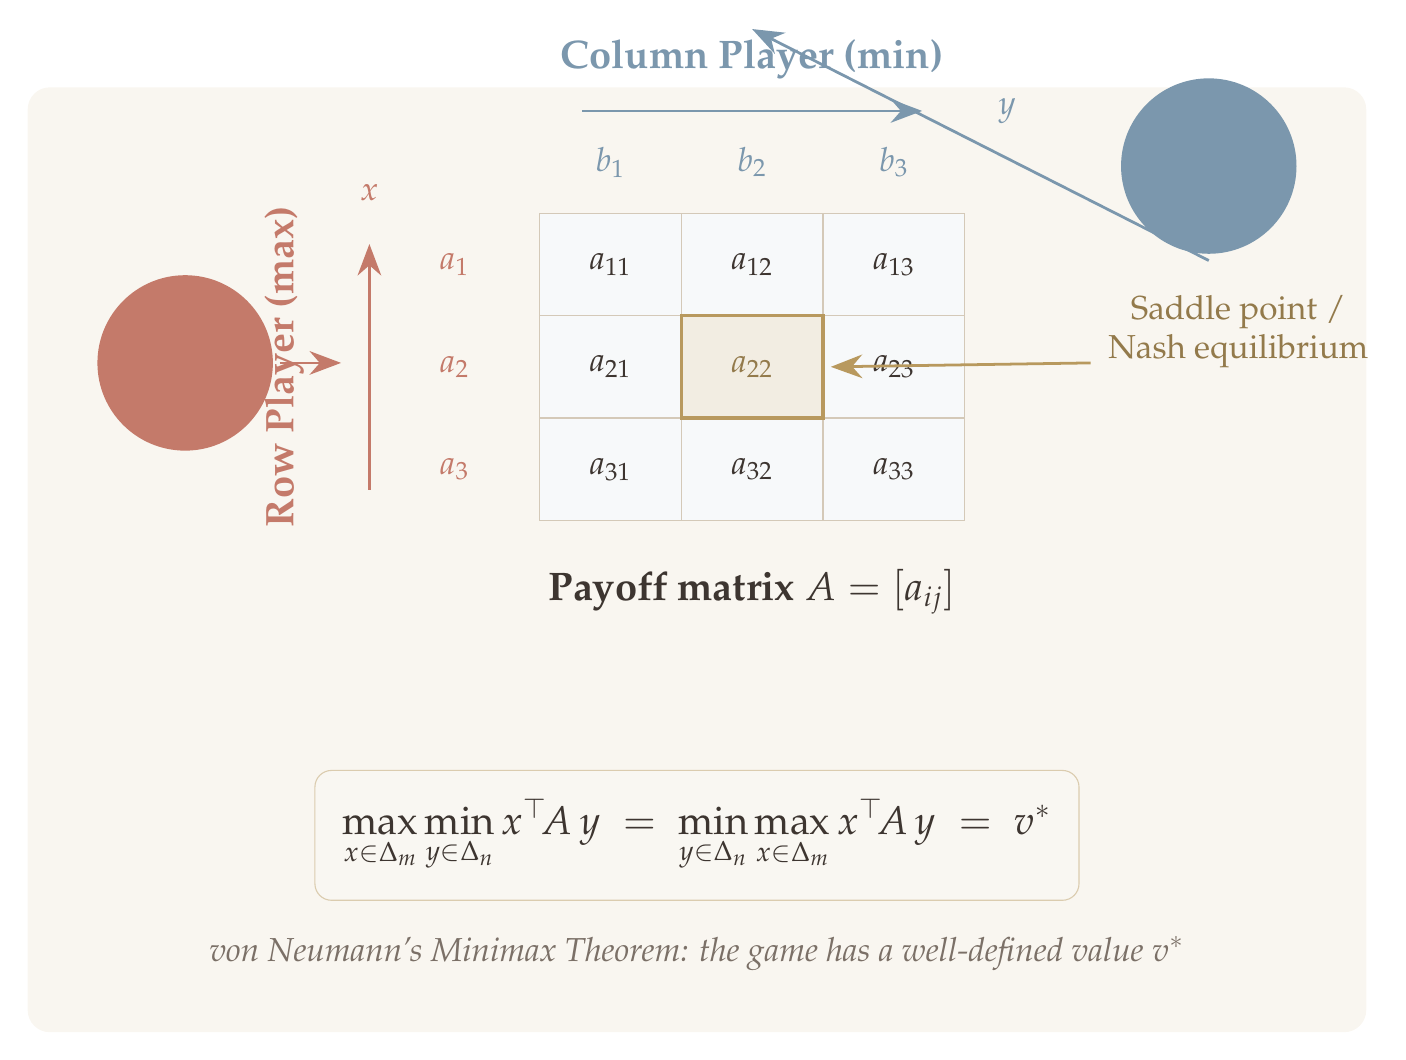
\begin{tikzpicture}[
    >={Stealth[length=4mm, width=3mm]},
    every node/.style={text=dkbrown},
  ]

  % Background
  \fill[cream, rounded corners=8pt] (-5.5,-5.5) rectangle (11.5,6.5);

  % === Payoff Matrix ===
  \def\cellw{1.8}
  \def\cellh{1.3}
  \def\ox{1.0}
  \def\oy{1.0}

  % Draw grid cells (3x3)
  \foreach \i in {0,1,2} {
    \foreach \j in {0,1,2} {
      \pgfmathsetmacro{\x}{\ox + \j*\cellw}
      \pgfmathsetmacro{\y}{\oy + (2-\i)*\cellh}
      \fill[stblue!6] (\x,\y) rectangle (\x+\cellw, \y+\cellh);
      \draw[border, line width=0.5pt] (\x,\y) rectangle (\x+\cellw, \y+\cellh);
    }
  }

  % Highlight saddle point cell (i=1, j=1)
  \pgfmathsetmacro{\sx}{\ox + 1*\cellw}
  \pgfmathsetmacro{\sy}{\oy + 1*\cellh}
  \fill[rwgold!18] (\sx,\sy) rectangle (\sx+\cellw, \sy+\cellh);
  \draw[rwgold, line width=1.2pt] (\sx,\sy) rectangle (\sx+\cellw, \sy+\cellh);

  % Payoff entries
  \node[font=\large] at (\ox+0.5*\cellw, \oy+2.5*\cellh) {$a_{11}$};
  \node[font=\large] at (\ox+1.5*\cellw, \oy+2.5*\cellh) {$a_{12}$};
  \node[font=\large] at (\ox+2.5*\cellw, \oy+2.5*\cellh) {$a_{13}$};

  \node[font=\large] at (\ox+0.5*\cellw, \oy+1.5*\cellh) {$a_{21}$};
  \node[font=\large\bfseries, rwgold!80!black] at (\ox+1.5*\cellw, \oy+1.5*\cellh) {$a_{22}$};
  \node[font=\large] at (\ox+2.5*\cellw, \oy+1.5*\cellh) {$a_{23}$};

  \node[font=\large] at (\ox+0.5*\cellw, \oy+0.5*\cellh) {$a_{31}$};
  \node[font=\large] at (\ox+1.5*\cellw, \oy+0.5*\cellh) {$a_{32}$};
  \node[font=\large] at (\ox+2.5*\cellw, \oy+0.5*\cellh) {$a_{33}$};

  % Column headers (Bob / min-player)
  \node[font=\large\bfseries, stblue] at (\ox+0.5*\cellw, \oy+3.5*\cellh) {$b_1$};
  \node[font=\large\bfseries, stblue] at (\ox+1.5*\cellw, \oy+3.5*\cellh) {$b_2$};
  \node[font=\large\bfseries, stblue] at (\ox+2.5*\cellw, \oy+3.5*\cellh) {$b_3$};

  % Column player label
  \node[font=\Large\bfseries, stblue] at (\ox+1.5*\cellw, \oy+4.5*\cellh) {Column Player (min)};
  \draw[->, stblue, line width=1pt] (\ox+0.3*\cellw, \oy+4.0*\cellh)
    -- (\ox+2.7*\cellw, \oy+4.0*\cellh);
  \node[font=\large, stblue] at (\ox+3.3*\cellw, \oy+4.0*\cellh) {$y$};

  % Row headers (Alice / max-player)
  \node[font=\large\bfseries, terracotta] at (\ox-0.6*\cellw, \oy+2.5*\cellh) {$a_1$};
  \node[font=\large\bfseries, terracotta] at (\ox-0.6*\cellw, \oy+1.5*\cellh) {$a_2$};
  \node[font=\large\bfseries, terracotta] at (\ox-0.6*\cellw, \oy+0.5*\cellh) {$a_3$};

  % Row player label
  \node[font=\Large\bfseries, terracotta, rotate=90] at (\ox-1.8*\cellw, \oy+1.5*\cellh)
    {Row Player (max)};
  \draw[->, terracotta, line width=1pt] (\ox-1.2*\cellw, \oy+0.3*\cellh)
    -- (\ox-1.2*\cellw, \oy+2.7*\cellh);
  \node[font=\large, terracotta] at (\ox-1.2*\cellw, \oy+3.2*\cellh) {$x$};

  % Matrix label
  \node[font=\Large\bfseries, text=dkbrown] at (\ox+1.5*\cellw, \oy-0.7*\cellh)
    {Payoff matrix $A = [a_{ij}]$};

  % Saddle point annotation
  \draw[->, rwgold, line width=1pt]
    (8.0, 3.0) -- (\sx+\cellw+0.1, \sy+0.5*\cellh);
  \node[font=\large, rwgold!80!black, align=center, anchor=west] at (8.1, 3.4)
    {Saddle point /\\Nash equilibrium};

  % === Minimax Theorem ===
  \node[font=\Large, text=dkbrown, align=center,
        fill=rwgold!8, draw=rwgold!50, rounded corners=6pt,
        inner sep=10pt] at (3.0, -3.0)
    {$\displaystyle \max_{x \in \Delta_m} \min_{y \in \Delta_n} x^\top\! A\, y
      \;=\; \min_{y \in \Delta_n} \max_{x \in \Delta_m} x^\top\! A\, y
      \;=\; v^*$};

  \node[font=\large\itshape, text=wmgray] at (3.0, -4.5)
    {von Neumann's Minimax Theorem: the game has a well-defined value $v^*$};

  % Row player icon (left)
  \node[circle, fill=terracotta!15, draw=terracotta, line width=0.8pt,
        minimum size=2.2cm, font=\large\bfseries, align=center, terracotta]
    at (-3.5, 3.0) {Max\\Player};

  % Column player icon (top-right)
  \node[circle, fill=stblue!12, draw=stblue, line width=0.8pt,
        minimum size=2.2cm, font=\large\bfseries, align=center, stblue]
    at (9.5, 5.5) {Min\\Player};

  % Arrows from players to matrix
  \draw[->, terracotta, line width=1pt] (-2.3, 3.0) -- (\ox-1.4*\cellw, 3.0);
  \draw[->, stblue, line width=1pt] (9.5, 4.3) -- (\ox+1.5*\cellw, \oy+4.8*\cellh);

\end{tikzpicture}
\end{document}
